\documentclass[10pt]{article}

% ---- NeurIPS-like single-column layout (self-contained; no external conference .sty) ----
\usepackage[letterpaper,left=1.5in,right=1.5in,top=1in,bottom=1in]{geometry}
\usepackage{mathptmx}            % Times text + math (NeurIPS look)
\usepackage[T1]{fontenc}
\usepackage{amsmath,amssymb}
\usepackage{graphicx}
\usepackage{booktabs}
\usepackage{array}
\usepackage{xcolor}
\usepackage[numbers]{natbib}
\usepackage{url}
\usepackage[hidelinks]{hyperref}

\setlength{\parindent}{0pt}
\setlength{\parskip}{0.5em}

% visible marker for content still to be filled with real numbers
\newcommand{\todo}[1]{{\color{red}\textbf{[TODO: #1]}}}

% NeurIPS-style abstract block
\renewenvironment{abstract}{%
  \vspace{0.5em}\begin{center}\rule{\textwidth}{0.5pt}\end{center}\vspace{-0.3em}
  {\centering\textbf{Abstract}\par}\vspace{0.3em}
  \begin{quote}\small}{%
  \end{quote}\vspace{-0.3em}\begin{center}\rule{\textwidth}{0.5pt}\end{center}}

\title{\textbf{Over-Squashing {\itshape vs.} Adversarial Robustness in GNNs:\\
An ``Add {\itshape vs.} Remove Edge'' Investigation}}
\author{
  Supanut Kompayak (st126055) \quad Dechathon Niamsa-Ard (st126235)\\
  Deep Learning Course Project, Asian Institute of Technology\\
  \texttt{\{st126055, st126235\}@ait.asia}
}
\date{Final Report --- \today}

\begin{document}
\maketitle

\begin{abstract}
% NOTE (final): update the last two sentences with the actual headline finding once Task 2--5 land.
Graph neural networks (GNNs) suffer from two seemingly unrelated structural problems: \emph{over-squashing},
where long-range information is compressed through bottlenecks and lost, and \emph{adversarial fragility},
where a few maliciously edited edges flip predictions. Both concern how sensitive a node's output is to
structural change elsewhere. As a learning project, we \emph{investigate} whether methods that mitigate
over-squashing also help adversarial robustness, through the lens of \textbf{adding vs.\ removing edges}:
over-squashing rewiring methods either \emph{add} edges (FoSR) or \emph{remove} them (spectral pruning),
while adversarial attacks add edges and adversarial defenses (GCN-Jaccard) remove them. On Cora and
Citeseer node classification we compare a vanilla GCN, an add-based rewiring (FoSR), a remove-based
spectral pruning (Jamadandi ProxyDelete), and two purpose-built defenses (GCN-Jaccard, GCN-SVD) under the
Metattack poisoning attack, reporting clean accuracy, robust accuracy, and the robustness gap, plus a
Jacobian-based over-squashing probe, an edge-overlap mechanism analysis, and a defense-aware attack. We
report only real, reproducible numbers; negative results are acceptable. We find that over-squashing
mitigations do \emph{not} transfer to robustness --- both add-based FoSR and spectral remove-based
ProxyDelete behave like an undefended GCN, while only the attack-aware defenses (GCN-Jaccard, GCN-SVD)
improve robustness --- indicating that the editing \emph{criterion}, not the add/remove direction,
governs robustness on this testbed.

\end{abstract}

\section{Introduction}
Message-passing GNNs propagate information hop-by-hop along edges. Two known failure modes both stem from
how information flows through graph structure. \textbf{Over-squashing}~\citep{alon2021bottleneck,
topping2022understanding,digiovanni2023oversquashing}: reaching distant nodes requires many layers, but the
exponentially growing long-range signal is squeezed through structural bottlenecks into a fixed-size vector
and lost --- the output is \emph{not sensitive enough} to distant signal. \textbf{Adversarial
fragility}~\citep{zugner2019metattack,zugner2018nettack}: an attacker adds or removes a few edges and message
passing pulls in the bad signal, flipping the prediction --- the output is \emph{too sensitive} to malicious
structural change. Both are about the sensitivity of a node's output to structural change elsewhere; this
conceptual bridge is what we investigate, not a claim we prove.

The sharper framing we use is \textbf{add vs.\ remove edge}. Over-squashing rewiring mostly \emph{adds} edges
to raise the spectral gap and relieve bottlenecks (FoSR~\citep{karhadkar2023fosr},
SDRF~\citep{topping2022understanding}); adversarial attacks typically \emph{add} edges between dissimilar
nodes; adversarial defenses \emph{remove} suspicious edges (GCN-Jaccard~\citep{wu2019jaccard},
Pro-GNN~\citep{jin2020prognn}). Thus adding edges to fix over-squashing might \emph{hurt} robustness (more
edges to exploit), while a \emph{remove}-based over-squashing method --- spectral
pruning~\citep{jamadandi2024spectral} --- might transfer to robustness because it removes edges like a defense
does. ``Add vs.\ remove: which helps robustness, and why?'' is the spine of this project.

\section{Related Work and Positioning}
The building blocks are established. Over-squashing is characterized by \citet{alon2021bottleneck},
\citet{topping2022understanding} and \citet{digiovanni2023oversquashing}, and mitigated by spectral
rewiring that \emph{adds} edges (FoSR~\citep{karhadkar2023fosr}) or \emph{deletes} them
~\citep{jamadandi2024spectral}. Structural adversarial attacks and defenses are equally well studied:
Metattack~\citep{zugner2019metattack} and Nettack~\citep{zugner2018nettack} perturb the graph, and
GCN-Jaccard~\citep{wu2019jaccard} defends by pruning edges between dissimilar nodes --- \citet{wu2019jaccard}
report that attacks ``tend to connect the target node to nodes with different features'' and that the
defense removes ``edges that connect nodes with low similarity.''

What is missing is the \emph{link} between the two lines of work, which motivates our study. To our
knowledge the interaction is unstudied: a current, comprehensive rewiring
survey~\citep{attali2024rewiringsurvey} does not mention adversarial robustness at all, and the
spectral-rewiring methods we use~\citep{karhadkar2023fosr, jamadandi2024spectral} neither evaluate nor
discuss it; conversely the GNN-robustness literature~\citep{wu2019jaccard, foth2025gtrobust} does not
engage over-squashing mitigation. The question is natural because the operations \emph{collide}:
over-squashing rewiring adds edges to raise connectivity --- structurally the same move an attacker makes
--- so whether it helps or hurts robustness is a priori unclear. A recent position
paper~\citep{kormann2026position} independently argues over-squashing mitigations bring limited practical
gains, echoing our robustness-side result, and the closest related method,
GraphTorque~\citep{huang2025graphtorque}, improves robustness by edge \emph{removal} --- consistent with
our finding that removal, not addition, helps. We contribute the controlled add-vs-remove study that
connects these threads; as a learning project, the contribution is the question and its controlled
empirical answer, not any new method.

\section{Research Questions}
\begin{itemize}
  \item \textbf{RQ2 (lead).} Do over-squashing mitigations (add-based FoSR vs.\ remove-based spectral pruning)
  improve adversarial robustness relative to (a) an undefended GCN and (b) a purpose-built defense
  (GCN-Jaccard), and at what cost to clean accuracy?
  \item \textbf{RQ1 (secondary).} Does structural perturbation measurably worsen an over-squashing measure?
  Is there a relationship between perturbation strength and long-range information loss?
  \item \textbf{RQ3 (stretch).} Can a single measure (Jacobian sensitivity) capture both over-squashing
  severity and adversarial fragility on the same scale?
\end{itemize}

\section{Data}
Cora is the workhorse; everything else is optional. All statistics are confirmed at load time.

\begin{table}[h]
\centering\small
\begin{tabular}{@{}llll@{}}
\toprule
\textbf{Dataset} & \textbf{Task} & \textbf{Size} & \textbf{Role} \\
\midrule
Cora (Planetoid)     & node clf.         & 2{,}708 nodes / 5{,}278 undir.\ edges / 7 cls / 1{,}433 feat & \textbf{primary} \\
Citeseer (Planetoid) & node clf.         & 3{,}327 / 4{,}552 / 6 / 3{,}703                              & 2nd setting \\
Peptides-func (LRGB) & graph clf.\ (AP)  & 15{,}535 graphs, $\sim$150 avg nodes                         & stretch \\
ZINC (subset)        & graph reg.\ (MAE) & 12{,}000 graphs, $\sim$23 avg nodes                          & stretch \\
\bottomrule
\end{tabular}
\caption{Datasets. Cora is the primary node-level and standard adversarial-attack testbed.}
\end{table}

\section{Methods and Approach}
\paragraph{Backbone.} GCN~\citep{kipf2017gcn} (2 layers, hidden $16$, dropout $0.5$). GAT/GraphSAGE are stretch.

\paragraph{The method table (the design).} Each method occupies a position on the add/remove axis:

\begin{table}[h]
\centering\small
\begin{tabular}{@{}llll@{}}
\toprule
\textbf{Method} & \textbf{Targets} & \textbf{Edge op} & \textbf{Role} \\
\midrule
GCN (vanilla)                  & ---                 & none            & baseline \\
FoSR                           & over-squashing      & \textbf{add}    & the ``add'' arm \\
Spectral pruning (ProxyDelete) & over-squashing      & \textbf{remove} & the ``remove'' arm \\
GCN-Jaccard                    & adversarial defense & \textbf{remove} & defense ref.\ (similarity) \\
GCN-SVD                        & adversarial defense & low-rank        & defense ref.\ (low-rank) \\
DropEdge                       & regularization      & remove (random) & random-removal sanity baseline \\
\bottomrule
\end{tabular}
\caption{\emph{FoSR vs.\ ProxyDelete} isolates the add/remove \emph{direction}; \emph{ProxyDelete vs.\ the
defenses} isolates the removal/edit \emph{criterion} (spectral vs.\ similarity vs.\ low-rank); \emph{all
vs.\ vanilla} asks whether any of this helps robustness, and at what clean-accuracy cost. GCN-SVD is a
second, mechanism-distinct defense reference.}
\end{table}

\paragraph{Attack and defense.} Metattack~\citep{zugner2019metattack}, a global meta-learning poisoning
attack, at perturbation rates $\{0.05, 0.10\}$. Defense reference: GCN-Jaccard~\citep{wu2019jaccard}. Both
via DeepRobust~\citep{li2021deeprobust}. Remove-based over-squashing arm: ProxyDelete spectral
pruning~\citep{jamadandi2024spectral} (deletes edges to maximize the spectral gap). Add-based arm:
FoSR~\citep{karhadkar2023fosr}, adapted from graph- to node-classification.

\paragraph{Pipeline order (the operational spine).} Metattack is a \emph{poisoning} attack, so operation
order is part of the design:
\[
\text{clean graph} \xrightarrow{\text{Metattack}} \text{poisoned } G'
\xrightarrow{\;M\;} G'' \xrightarrow{\text{train GCN}} \text{eval}.
\]
The transform $M \in \{\text{none, FoSR, ProxyDelete, GCN-Jaccard}\}$. A method changes the graph even with
no attack, giving four conditions per method: clean; clean${+}M$; poisoned; poisoned${+}M$.

\paragraph{Over-squashing probe.} Jacobian sensitivity $\partial \mathbf{h}_v / \partial \mathbf{x}_u$ for
distant pairs $(u,v)$~\citep{digiovanni2023oversquashing}, via autograd (scoped to a few far pairs first).

\section{Experimental Setup}
All robustness experiments use DeepRobust's Cora with the standard \texttt{nettack} split (largest connected
component, $2485$ nodes). The poisoned adjacency is generated once per perturbation rate (Metattack,
\texttt{Meta-Self}, attack seed $15$) and cached; every method reuses it. Reported accuracies are mean $\pm$
std over $3$ training seeds on the fixed poisoned graph. Backbone hyperparameters: hidden $16$, dropout
$0.5$, lr $0.01$, weight decay $5\!\times\!10^{-4}$, $200$ epochs. Rewiring/removal methods share a matched
edge budget for the add/remove comparison; GCN-SVD uses rank $k{=}50$. All computation runs on CPU.
The main attacker is non-adaptive (it attacks a vanilla GCN surrogate, unaware of the defense); we probe
this assumption directly with a heuristic defense-aware attack (\S\ref{sec:results}, ``adaptive attacker'').

\section{Results}\label{sec:results}
\paragraph{Baseline.} On the standard Planetoid public split the vanilla GCN reaches $80.30 \pm 0.47\%$
(5 seeds). On the DeepRobust \texttt{nettack} split (2485 nodes, 3 seeds) it reaches $83.50 \pm 0.46\%$
clean, falling to $77.05\%$ and $71.85\%$ under Metattack at $\text{ptb}=0.05$ and $0.10$
(Table~\ref{tab:headline}).

\paragraph{Headline: add vs.\ remove under attack.} Table~\ref{tab:headline} reports the full grid, and
the result is decisive --- and largely negative for the over-squashing hypothesis. \emph{Only the two
purpose-built defenses improve robustness.} The undefended GCN, random removal (DropEdge), add-based
rewiring (FoSR) and spectral removal (ProxyDelete) all cluster together (robust accuracy $76.7$--$77.1\%$
at ptb $0.05$ and $71.0$--$71.9\%$ at ptb $0.10$), while GCN-Jaccard and GCN-SVD stand clearly apart.
Jaccard has the best low-perturbation robust accuracy ($78.84\%$) at a small clean cost ($\sim$1.3 pts);
GCN-SVD, via low-rank filtering, is the most attack-\emph{immune} (gap $0.4$/$2.3$; the best robust
accuracy at ptb $0.10$, $75.29\%$) though at a larger clean cost ($\sim$6 pts). FoSR and ProxyDelete show
marginally smaller \emph{gaps} than the vanilla GCN only because their clean accuracy is lower --- their
robust accuracy is not improved --- so the gap must be read alongside robust accuracy. Crucially,
\emph{the add/remove direction does not determine robustness}: both over-squashing methods fail to defend
whether they add (FoSR) or remove (ProxyDelete) edges. What separates the defenses is that both are
\emph{attack-aware} --- Jaccard removes the dissimilar-feature edges the attacker inserts, SVD filters the
high-rank perturbation --- whereas the over-squashing methods optimize a structural quantity (the spectral
gap) unrelated to the attack.

\begin{table}[h]
\centering\small
\begin{tabular}{@{}lccccc@{}}
\toprule
\textbf{Method} & \textbf{Clean} & \textbf{Robust@0.05} & \textbf{Robust@0.10} & \textbf{Gap@0.05} & \textbf{Gap@0.10} \\
\midrule
GCN (vanilla)              & $83.50${\scriptsize$\pm.46$} & $77.05${\scriptsize$\pm.51$} & $71.85${\scriptsize$\pm.72$} & $6.46$ & $11.65$ \\
FoSR (add)                 & $82.53${\scriptsize$\pm.13$} & $76.78${\scriptsize$\pm.60$} & $70.96${\scriptsize$\pm.55$} & $5.75$ & $11.57$ \\
ProxyDelete (spectral rm.) & $82.60${\scriptsize$\pm.07$} & $76.71${\scriptsize$\pm.52$} & $71.68${\scriptsize$\pm.68$} & $5.89$ & $10.92$ \\
DropEdge (random rm.)      & $83.17${\scriptsize$\pm.61$} & $76.98${\scriptsize$\pm.40$} & $71.40${\scriptsize$\pm.87$} & $6.19$ & $11.77$ \\
\midrule
GCN-Jaccard (similarity rm.) & $82.16${\scriptsize$\pm.39$} & $\mathbf{78.84}${\scriptsize$\pm.27$} & $74.45${\scriptsize$\pm.68$} & $3.32$ & $7.71$ \\
GCN-SVD (low-rank)         & $77.58${\scriptsize$\pm.41$} & $77.20${\scriptsize$\pm.14$} & $\mathbf{75.29}${\scriptsize$\pm.60$} & $\mathbf{0.39}$ & $\mathbf{2.30}$ \\
\bottomrule
\end{tabular}
\caption{Headline grid on Cora (test acc \%, \texttt{nettack} split, Metattack, 3 seeds). Lower gap $=$ more
robust. Top block: undefended GCN and the over-squashing/random arms; bottom block: the two purpose-built
defenses. Only the defenses separate from the vanilla-GCN level.}
\label{tab:headline}
\end{table}

\begin{figure}[h]
\centering
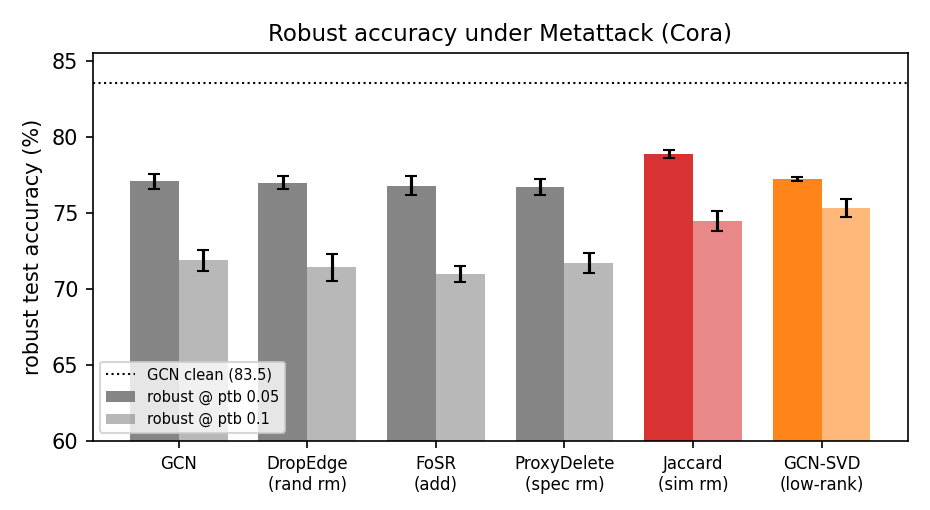
\includegraphics[width=0.72\textwidth]{figures/headline.png}
\caption{Robust accuracy per method under Metattack (Cora). The over-squashing and random arms cluster
at the vanilla-GCN level; only GCN-Jaccard (red) separates. Dotted line: clean GCN accuracy.}
\label{fig:headline}
\end{figure}

\paragraph{Why does Jaccard win? (mechanism).} Metattack here is almost purely edge-\emph{addition}
(it inserts $253$/$503$ edges at ptb $0.05$/$0.10$ and deletes $0$/$3$), which validates the add/remove
framing. Table~\ref{tab:overlap} then measures how many of those inserted edges each method deletes.
The story is mechanistic: GCN-Jaccard removes about \emph{half} of the attacker's edges (recall $0.50$,
$\sim$3.6$\times$ the chance rate of a random remover) --- it literally undoes the attack. Spectral
pruning removes attack edges only slightly above chance ($0.19$ vs.\ $0.12$), random DropEdge sits
exactly at chance, and FoSR (which only adds) removes none. Robustness therefore tracks \emph{how many
attacker edges a method deletes}, and only the similarity criterion deletes them at scale.

\begin{table}[h]
\centering\small
\begin{tabular}{@{}lcccc@{}}
\toprule
\textbf{Method} (ptb $0.10$) & \textbf{\# removed} & \textbf{attack edges rm.} & \textbf{recall} & \textbf{chance} \\
\midrule
GCN-Jaccard           & $797$ & $250$ & $\mathbf{0.50}$ & $0.14$ \\
ProxyDelete (spectral)& $643$ & $93$  & $0.19$ & $0.12$ \\
DropEdge (random)     & $643$ & $59$  & $0.12$ & $0.12$ \\
FoSR (add)            & $0$   & $0$   & $0.00$ & --- \\
\bottomrule
\end{tabular}
\caption{Edge-overlap mechanism (Cora, ptb $0.10$). \emph{Recall} $=$ fraction of the attacker's
inserted edges the method deletes; \emph{chance} $=$ recall of a random remover of the same size. Only
Jaccard removes attack edges far above chance --- explaining why only it defends.}
\label{tab:overlap}
\end{table}

\paragraph{Do the methods raise the spectral gap? (sanity).} The over-squashing methods do exactly what
they claim --- it just does not help. On clean Cora the normalized-Laplacian spectral gap ($\lambda_2$)
is $0.005$; the poisoning attack itself \emph{raises} it to $0.016$ (adding edges improves connectivity),
and FoSR raises it further to $0.054$, a $3.3\times$ increase over the poisoned graph. Yet neither buys
robustness --- the attack lowers accuracy and FoSR leaves it unchanged. Raising the spectral gap, the
explicit objective of over-squashing rewiring, is thus uncorrelated (here even anti-correlated) with
robustness, so the methods are working as intended on the wrong quantity. (Removal-based methods can
fragment the graph, making $\lambda_2$ degenerate, so we make this point on the add side; the removal
side is covered by the edge-overlap analysis above.)

\paragraph{Over-squashing probe (RQ1).} Figure~\ref{fig:probe} plots the mean Jacobian sensitivity
$\|\partial h_v/\partial x_u\|_F$ of a 6-layer GCN against graph distance $d(u,v)$. The over-squashing
signature is unmistakable: sensitivity decays roughly geometrically, about $5\times$ per hop (from $4.0$
at $d{=}1$ to $7\!\times\!10^{-4}$ at $d{=}6$ on the clean graph), so distant nodes have almost no
influence on a node's output. Comparing the clean and poisoned ($\text{ptb}=0.10$) graphs, the per-hop
decay rate is essentially unchanged; poisoning lowers the overall magnitude but does not steepen the
long-range decay. Thus structural attack does not worsen the over-squashing \emph{measure} itself at
these perturbation levels --- consistent with the RQ2 finding that the two phenomena are governed by
different factors. (Absolute magnitudes depend on the separately trained weights, so the decay
\emph{slope} is the reliable comparison; a weight-controlled variant is a natural follow-up.)

\begin{figure}[h]
\centering
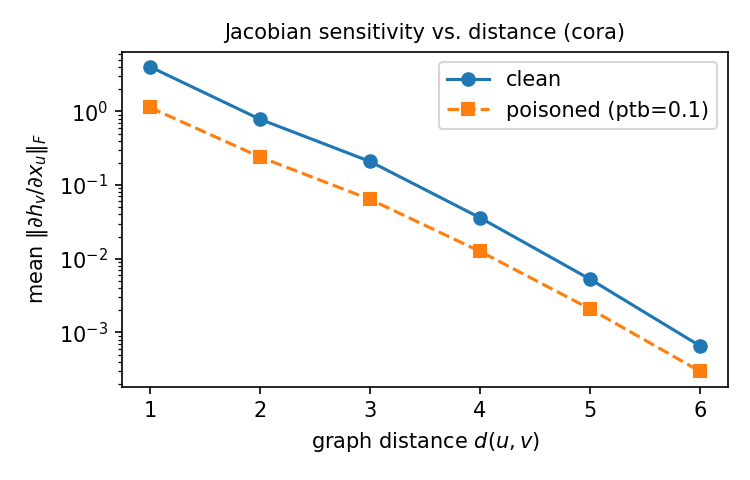
\includegraphics[width=0.6\textwidth]{figures/probe.png}
\caption{Jacobian sensitivity $\|\partial h_v/\partial x_u\|_F$ vs.\ graph distance (6-layer GCN, Cora;
log scale). The $\sim$geometric decay is the over-squashing signature; clean and poisoned graphs share
the same decay rate.}
\label{fig:probe}
\end{figure}

\paragraph{Second dataset (Citeseer).} The pattern generalizes (Table~\ref{tab:citeseer}). Citeseer is
naturally more robust here --- the attack opens only a $1.9$/$4.2$-point gap on the vanilla GCN --- but
the ordering is identical: GCN-Jaccard is again strongest, with the highest robust accuracy
($70.97$/$68.40\%$) and smallest gap ($1.03$/$3.59$), while spectral removal (ProxyDelete,
$68.82$/$66.82$) and add-based rewiring (FoSR, $69.33$/$65.36$) do not help --- FoSR again hurts at the
higher perturbation rate. Random removal (DropEdge) tracks the vanilla GCN. As on Cora, only
similarity-targeted removal improves robustness.

\begin{table}[h]
\centering\small
\begin{tabular}{@{}lccccc@{}}
\toprule
\textbf{Method} & \textbf{Clean} & \textbf{Robust@0.05} & \textbf{Robust@0.10} & \textbf{Gap@0.05} & \textbf{Gap@0.10} \\
\midrule
GCN (vanilla)        & $71.84$ & $69.94$ & $67.69$ & $1.90$ & $4.15$ \\
FoSR (add)           & $71.23$ & $69.33$ & $65.36$ & $1.90$ & $5.86$ \\
ProxyDelete (remove) & $71.60$ & $68.82$ & $66.82$ & $2.78$ & $4.78$ \\
GCN-Jaccard (remove) & $72.00$ & $\mathbf{70.97}$ & $\mathbf{68.40}$ & $\mathbf{1.03}$ & $\mathbf{3.59}$ \\
DropEdge (random)    & $71.64$ & $69.67$ & $67.65$ & $1.97$ & $3.99$ \\
\bottomrule
\end{tabular}
\caption{Citeseer headline grid (test acc \%, \texttt{nettack} split, Metattack, 3 seeds). The Cora
conclusion holds: only GCN-Jaccard improves robustness.}
\label{tab:citeseer}
\end{table}

\paragraph{An adaptive (defense-aware) attacker.} Our attacker so far is non-adaptive. Since Jaccard
removes edges between \emph{dissimilar} nodes, a defense-aware attacker should instead add edges between
feature-\emph{similar} but differently-labelled nodes, which the filter cannot remove. We built exactly
such a heuristic evasion attack. It succeeds at the filter level --- Jaccard removes $0\%$ of its inserted
edges --- so the defense is, in principle, evadable. But the evasion is largely self-defeating: forcing
edges to be similarity-high drastically weakens the attack, dropping vanilla-GCN accuracy by only
$0.7$/$2.1$ points at budget $253$/$503$, versus $6.5$/$11.7$ for Metattack at comparable budgets. The
edges that fool the model (dissimilar) are exactly the ones Jaccard removes, while the edges that evade
Jaccard (similar) barely fool the model --- attack potency and detectability are coupled. (Jaccard even
slightly \emph{hurts} here, paying its clean-accuracy cost while removing none of the evasion edges.) This
is a heuristic, not gradient-optimal, adaptive attack; a jointly optimized adaptive attack remains future
work.

\section{Discussion}
The grid answers RQ2 directly. The attacker mostly \emph{adds} dissimilar edges; GCN-Jaccard \emph{removes}
exactly those (which is why removal defends); FoSR \emph{adds} more edges; ProxyDelete \emph{removes} edges by
a spectral criterion. \emph{FoSR vs.\ ProxyDelete} isolates edge direction; \emph{ProxyDelete vs.\
GCN-Jaccard} isolates the removal criterion. Our working hypothesis was that add-based rewiring is
neutral-to-harmful for robustness while remove-based pruning partially transfers. The data only half match
it: add-based FoSR is indeed neutral-to-harmful, but \emph{remove-based spectral pruning does not transfer
either} --- ProxyDelete behaves like the vanilla GCN, not like the defense. The discriminating factor is
therefore not the add/remove \emph{direction} but the removal \emph{criterion}: only similarity-targeted
removal (Jaccard), which directly undoes the attacker's dissimilar-edge insertions --- deleting
$\sim$50\% of them versus near-chance for the spectral and random arms (Table~\ref{tab:overlap}) ---
improves robustness, while spectral-gap-guided editing (add or remove) does not. On this testbed the conceptual bridge between
over-squashing and adversarial robustness is \emph{not} supported: mitigating over-squashing does not buy
robustness. A natural worry is budget: Jaccard removes $\sim$643 edges (similarity-threshold-driven)
versus the $253$ matched across the spectral/random arms. Equalizing it does not change the verdict ---
at a $643$-edge budget, ProxyDelete still reaches only $76.9$/$71.3\%$ robust (vs.\ Jaccard's
$78.8$/$74.5\%$), while removing $643$ random edges (DropEdge, $76.5$/$70.9$) or adding $643$ (FoSR,
$76.3$/$69.9$) does not help and can hurt. The gap to Jaccard is therefore driven by the removal
\emph{criterion}, not the edge budget.

\section{Conclusion}
On a controlled add-vs-remove grid (Cora, Metattack), over-squashing mitigations did not improve
adversarial robustness: add-based FoSR and spectral remove-based ProxyDelete both tracked the undefended
GCN ($\approx$$77\%$/$72\%$ robust at ptb $0.05$/$0.10$), while only purpose-built, attack-aware defenses
did --- GCN-Jaccard (similarity pruning) and GCN-SVD (low-rank filtering) --- through two distinct
mechanisms. The discriminating factor is the editing \emph{criterion}, not the add/remove direction or
edge count: robustness here comes from targeting the attacker's perturbation (dissimilar edges / high-rank
structure), not from optimizing the spectral gap. On this testbed, then, the over-squashing$\to$robustness
bridge is not supported --- an honest negative result, and one that replicates on Citeseer
(Table~\ref{tab:citeseer}). A heuristic defense-aware attacker can evade Jaccard's filter but only by
becoming much weaker, suggesting attack potency and detectability are coupled. The Jacobian probe confirms
over-squashing is present (sensitivity decays $\sim$$5\times$ per hop) yet shows poisoning does not steepen
that decay (RQ1), reinforcing that the two phenomena are decoupled. Future work: a gradient-optimal
adaptive attack, and testing whether a single Jacobian measure tracks both phenomena (RQ3).

\paragraph{Reproducibility.} All numbers are produced by fixed-seed scripts and are reproducible end-to-end;
poisoned graphs are cached and every table regenerates from a single command. We report only real, measured
results.

\bibliographystyle{plainnat}
\bibliography{references}

\appendix
\section{Implementation Notes}
DeepRobust ($0.2.9$) installed with \texttt{--no-deps} (to avoid a broken \texttt{gensim} pin) plus prebuilt
PyG extension wheels (\texttt{torch\_sparse}, \texttt{torch\_scatter}) matched to torch~$2.9$/cu128; all
compute on CPU. Full Metattack (\texttt{Meta-Self}) on Cora costs $\sim$37~min at $\text{ptb}=0.05$ on CPU,
hence the precompute-and-cache design.

\section{Budget-matched robustness check}
To rule out that Jaccard's advantage is merely a larger edit budget, we re-ran the remove/add arms with a
budget of $643$ edges (matching Jaccard's similarity-threshold count) instead of the $253$ used in
Table~\ref{tab:headline}. Robust accuracy is essentially unchanged: the criterion, not the budget, drives
the defense.

\begin{table}[h]
\centering\small
\begin{tabular}{@{}lccc@{}}
\toprule
\textbf{Method (budget $643$)} & \textbf{Clean} & \textbf{Robust@0.05} & \textbf{Robust@0.10} \\
\midrule
GCN (vanilla)        & $83.50$ & $77.05$ & $71.85$ \\
GCN-Jaccard ($\sim$643) & $82.16$ & $\mathbf{78.84}$ & $\mathbf{74.45}$ \\
ProxyDelete (remove) & $82.03$ & $76.89$ & $71.28$ \\
DropEdge (random)    & $81.66$ & $76.48$ & $70.88$ \\
FoSR (add)           & $82.26$ & $76.32$ & $69.89$ \\
\bottomrule
\end{tabular}
\caption{Budget-matched check (Cora, test acc \%, 3 seeds). Even at Jaccard's $\sim$643-edge budget,
spectral/random/add arms stay at the vanilla-GCN level; only Jaccard defends.}
\end{table}

\end{document}
